\section{Datensatz}
\label{sec:datensatz}
\subsection{Erzeugung}
Der Datensatz besteht aus einem Satellitenbild und einer 'Maske'.
'Maske' steht dabei für eine Karte, in der ausschließlich Gewässer eingezeichnet sind.
\\
Zur Verdeutlichung ist in \autoref{fig:datensatz} ein Satellitenbild und die zugehörige Maske eines Flusses in Litauen dargestellt.
\begin{figure}
    \begin{subfigure}{0.48\textwidth}
        \centering
        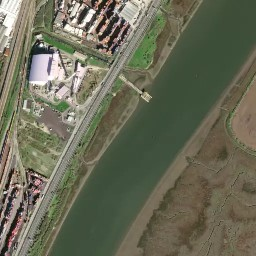
\includegraphics[width=\textwidth]{content/img/datensatz_satellite.jpg}
        \caption{Satellitenbild}
    \end{subfigure}
    \hfill
    \begin{subfigure}{0.48\textwidth}
        \centering
        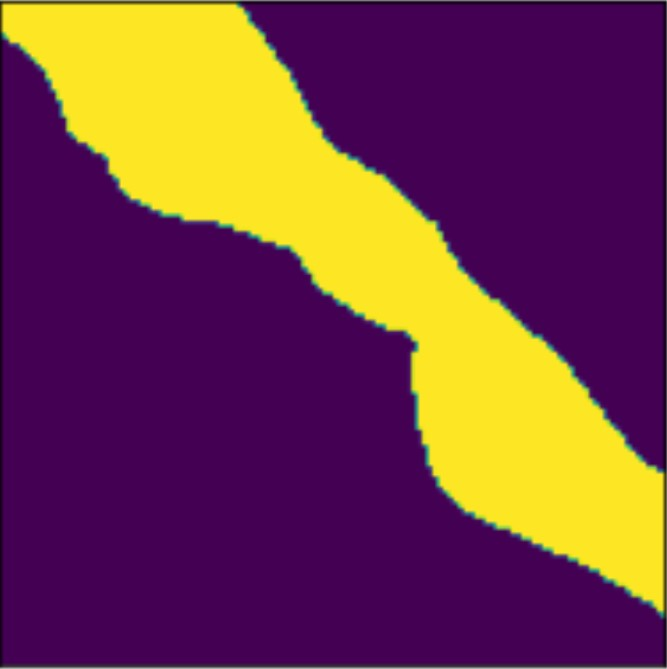
\includegraphics[width=\textwidth]{content/img/datensatz_mask.jpg}
        \caption{Maske}
    \end{subfigure}
    \caption{Beispiel aus dem Datensatz für ein Satellitenbild aus Littauen mit zugehöriger Maske.\cite{mapbox}}
    \label{fig:datensatz}
\end{figure}
\\
Der Datensatz wird mit Python über die API von Mapbox\cite{mapbox} generiert.
Europa hat einen Wasserflächenanteil von wenigen Prozent.
Um nun nicht größtenteils gewässerfreie Satellitenaufnahmen zu erhalten, muss geprüft werden ob sich in den gezogenen Koordinaten ein Fluss, See oder Meer befindet.
Die Erzeugung des Datensatzes kann in folgende Schritte unterteilt werden:
\begin{itemize}
    \item generiere zufällige Längen- und Breitengrade auf dem europäischen Festland (Ländergrenzen aus 'Natural Earth' \cite{naturalearth})
    \item prüfe ob Gewässer innerhalb eines 'Tiles'\footnote{\label{foot:tiles}Die Karte wird Abhängig von der Zoomstufe in unterschiedlich viele Quadrate unterteilt, sog. 'Tiles'.} vorkommen
    \item Download des Satelliten- und Maskenbilds über die Mapbox API\cite{mapbox} \\
          per Link: \url{https://api.mapbox.com/v4/mapbox.satellite/{zoom}/{lon}/{lat}.mvt?access_token=\{token\}}
    \item skaliere Bilder von $256 \, \text{px} \times 256 \, \text{px}$ zu $128 \, \text{px} \times 128 \, \text{px}$
\end{itemize}
Die zufällig erzeugten Längen- und Breitengrade werden im Bereich
\begin{align*}
    \SI{-10.49}{\degree} &< lon < \SI{40.27}{\degree} \\
    \SI{34.51}{\degree} &< lat < \SI{71.20}{\degree}
\end{align*}
gezogen, somit wird Russland und Island vorweg ausgeschlossen.
Zu den akzeptierten Koordinaten, also Satellitenbilder die Gewässer abbilden wird ebenfalls das Land mithilfe von Shapely\cite{shapely} ermittellt.
\\
Zum Download der Bilder müssen die zuvor generierten Längen- und Breitengrade und zum anderen der Zoom-Faktor angegeben werden.
Umso größer der Zoom-Faktor, desto kleinere Gewässer können erkannt werden, doch desto größer ist die Wahrscheinlichkeit Satellitenbilder auschließlich mit Wasser zu erhalten.
Mit dem gewählten Zoom-Faktor $Z = 15$ liegt der Fokus auf Flüsse, mittelgroße/große Seen und Küstenabschnitte.
\\
Um die Laufzeit zu verkürzen wird die Anzahl der Pixel pro Bild um $\SI{75}{\percent}$ reduziert.

\subsection{Eigenschaften}
Der Datensatz beinhaltet $\SI{57931}{}$ Proben mit folgenden Informationen:
\begin{itemize}
    \item Längengrad
    \item Breitengrad
    \item Name des Landes
    \item Satellitenbild
    \item Maskenbild
\end{itemize}
Dabei erhält der Algorithmus das Satellitenbild als Input ($X$) und die Maske als Ziel ($Y$).
Die anderen Attribute geben den Ort der Aufnahme an, sind aber nicht für die eigentliche Problemstellung, sondern für die Reproduzierbarkeit notwendig.
\\
Das Satellitenbild liegt im 'JPEG'-Format vor, beinhaltet also die drei Farbchannel $RGB$ mit Werten von $0$ bis $255$.
\\
Hingegen wird für das Maskenbild das 'PNG'-Format verwendet.
Es handelt sich um Graustufenbilder mit einem Farbchannel, welcher Werte von $0$ bis $1$ annehmen kann.
\\
Wie bereits erwähnt beträgt die Auflösung für Masken- und Satellitenbild $128 \, \text{px} \times 128 \, \text{px}$.